\documentclass{article} 
\usepackage[T1]{fontenc}
\usepackage[utf8]{inputenc}
\usepackage{graphicx}       % Para imágenes
\usepackage{geometry}       
\usepackage{listings}  
\usepackage{hyperref}       
\usepackage{titling}        

\hypersetup{
    colorlinks= true,
    linkcolor= blue,
    urlcolor=blue
}
\geometry{margin=1.5cm}


\title{Análisis y especificaciones de requisitos}

\author{Iván Alfaya Pérez}

\date{\today}


\newcommand{\subtitle}{Proyecto: Aplicacion Movil de gestor de usuarios} % Subtítulo

\posttitle{\par\vspace{0.5cm}\large \subtitle\end{center}\vskip 0.5cm} 
\begin{document}

\maketitle

% Imagen debajo del título
\begin{figure}[h!]
    \centering
    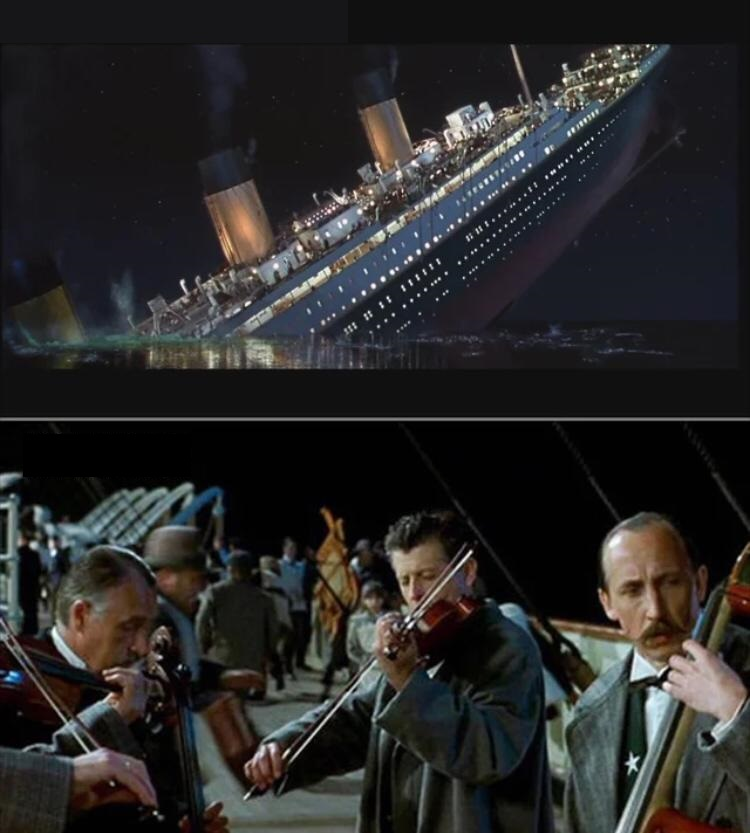
\includegraphics[width=0.7\textwidth]{img1.jpg}
\end{figure}

\clearpage 

\tableofcontents % Tabla de contenido
\clearpage 

\section{Descripcion de la app}
Se propone desarrolar una app para llevar la gestion de usuarios, y podran:
\begin{itemize}
    \item Creación de nuevos usuarios. 
    \item Eliminacion de nuevos usuarios.
    \item Modificacion de usuarios existentes.
    \item Mostrar todos los usuarios que tenemos.
    
\end{itemize}

\section{Requisitos}
A continuacion se listan los requisitos funcionales del sistema:

\begin{itemize}
    \item RF-1: El usuario podra consultar los diferentes usuarios de la app.
    \item RF-2: El usuario podra acceder a un formmulario para la creacion de nuevos usuarios.
    \item RF-3: El usuario podra borrar a un usuario con un boton en la targeta.
    \item RF-4: Al pulsar el boton de modificar se llenara un formulario con los datos del usuario y podras actualizar.
    \item RF-5: Al borrar o modificar tendra que salir un mensaje que preguntara si estas seguro de hacerlo o no(confirmacion).
\end{itemize}

\section{Requisistos no funcionales}

\begin{itemize}

    \item RNF-1: La interfaz debe ser intuitva y facil.
    \item RNF-2: Consistencia entre los colores tipografia e iconos.
    \item RNF-3: Los tiempos de carga no deben superar los 3 segs.
    \item RNF-4: Las acciones del usuario en la app no deben ser superiores a 2 segs.
    
\end{itemize}
\newpage
\section{Casos de usos}
\begin{figure}[h!]
    \centering
    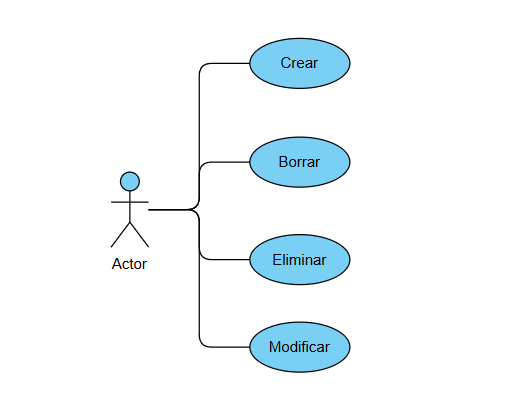
\includegraphics[width=0.7\textwidth]{diagramaUso.png}
\end{figure}

Descripcion de casos de usos principales.
\begin{table}[h!]
\centering
\begin{tabular}{|c|p{6cm}|} % la segunda columna de 6 cm
\hline
\textbf{Caso de uso} & \textbf{Descripción} \\
\hline
Crear nuevo usuario & El usuario accede al formulario de la creación, rellena los campos y guarda. \\
\hline
Borrar & El usuario elige a quien borrar, confirma que quiere borrar y borra. \\
\hline
Modificar & El usuario selecciona a quien modificar, aparece el formulario, modifica, confirma y guarda. \\
\hline
Mostrar & Se muestran todos los usuarios que existan. \\
\hline
\end{tabular}
\caption{Tabla de Usos}
\end{table}

\section{Historias de usuarios}

\begin{table}[h!]
\centering
\begin{tabular}{|c|p{3cm}|p{5cm}|p{4cm}|}
\hline
\textbf{ID} & \textbf{Como...} & \textbf{Quiero...} & \textbf{Para...} \\
\hline
HU-01 & Usuario & Crear un nuevo usuario & Añadir información de un nuevo usuario a la base de datos \\
\hline
HU-02 & Usuario & Ver todos los usuarios & Saber cuántos usuarios existen y consultar sus datos \\
\hline
HU-03 & Usuario & Modificar un usuario existente & Actualizar la información cuando sea necesario \\
\hline
HU-04 & Usuario & Borrar un usuario & Mantener la base de datos limpia y sin registros obsoletos \\
\hline
\end{tabular}
\caption{Historias de usuario para un CRUD}
\end{table}


\end{document}
